\section{Validation Croisée}

La validation croisée est une méthode d'évaluation qui consiste a moyenné les scores calculés sur plusieurs jeux de données pour un seul tuple de paramètre. (voir~\autoref{fig:Valid_Croisee})


\begin{figure}[htpb]
	\centering
	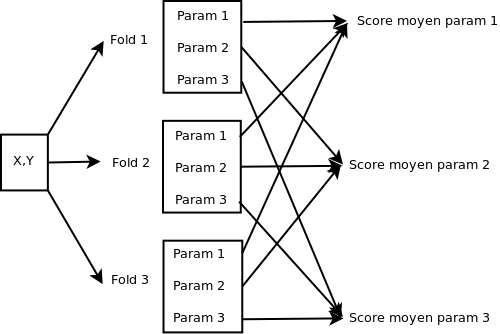
\includegraphics[scale = 0.25]{images/Valid_Croisee}
	\caption{Schéma de fonctionnement de la validation croisée}
	\label{fig:Valid_Croisee}
\end{figure}


Le principe de la validation croisée est de séparer un ensemble de donnée en plusieurs groupes de tailles équivalentes. Sur le schéma de la  \autoref{fig:Valid_Croisee_param}, on peut observer un ensemble de donné séparé en 3 avec $X_{1}$, $X_{2}$, $X_{3}$.
Chacun à tour de rôle sera utilisé pour l'apprentissage et le test. 
Sur les deux schémas, on peut lire "score", cela représente le résultat estimé par la régression linéaire. C'est ce même score qui sera comparé aux vrais score pour savoir si notre estimation est correcte et les résultats prédits bons. 
Il va sans dire que 

\begin{figure}[htpb]
	\centering
	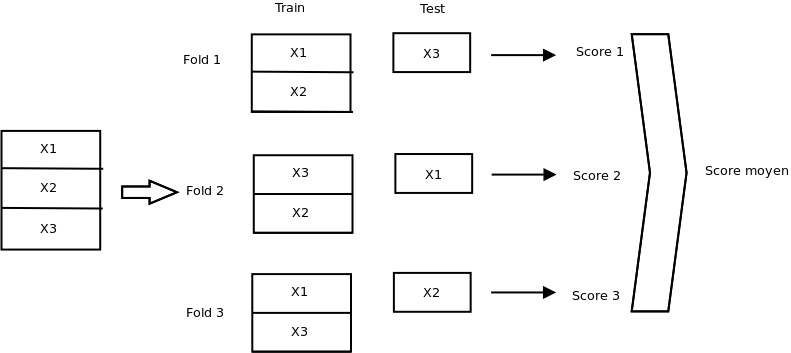
\includegraphics[scale = 0.25]{images/Valid_Croisee_param}
	\caption{Schéma de calcul d'un score par validation croisée}
	\label{fig:Valid_Croisee_param}
\end{figure}


Toutes les méthodes décrites dans cette partie représente enormément de temps de calculs. Pour réduire ce temps la, le module MapReduce va être utilisé. 